\section{Methodology}
Introduction goes here, no headline
train lottery tickets on simple task that contains independence.
\subsection{Idea}
The structure of lottery tickets is still mysterious. 
Analyzing the structure of a large and sparse Directed acyclic graph is not an easy task. 
However, one could approach the problem the other way around. 
Instead of analyzing the structure of an existing Lottery ticket, one could see what kind of structure appears given a problem with a known structure.
Inspired by the experiments in \autocite{BIMT}, a dataset that contains an independence problem was created.
The question is:
"Will a lottery ticket trained on an independece dataset result in seperate networks?"
In the course of this thesis, it is demonstrated that IMP indeed finds lottery tickets composed of two disconnected subnetworks inside a larger network.
\subsection{the independence dataset}
\textcite{BIMT} executed the experiements on symbolic regression datasets.
These are simple toy datasets where the labels are computed with a symbolic formula. 
For instance regarding the independence task, the inputs are $x_1, x_2, x_3, x_4$ and the outputs are $y_1={x_2}^2 + \sin{(\pi*x_4)}$ and $y_2=(x_1+x_3)^3$
In this case the independence is obvious, as $y_1$ depends only on $x_1$ and $x_3$, and $y_2$ depends only on $x_2$ and $x_4$.
However with regards to lottery tickets, the existing literature focuses on classification tasks, while this is a regression task.

Therefore instead of using the independence dataset from \autocite{BIMT}, a different dataset has to be created.

To create a simple toy classification task with independance, two classic toy datasets are concatenated into one dataset.
\begin{figure}[ht]
    \centering
    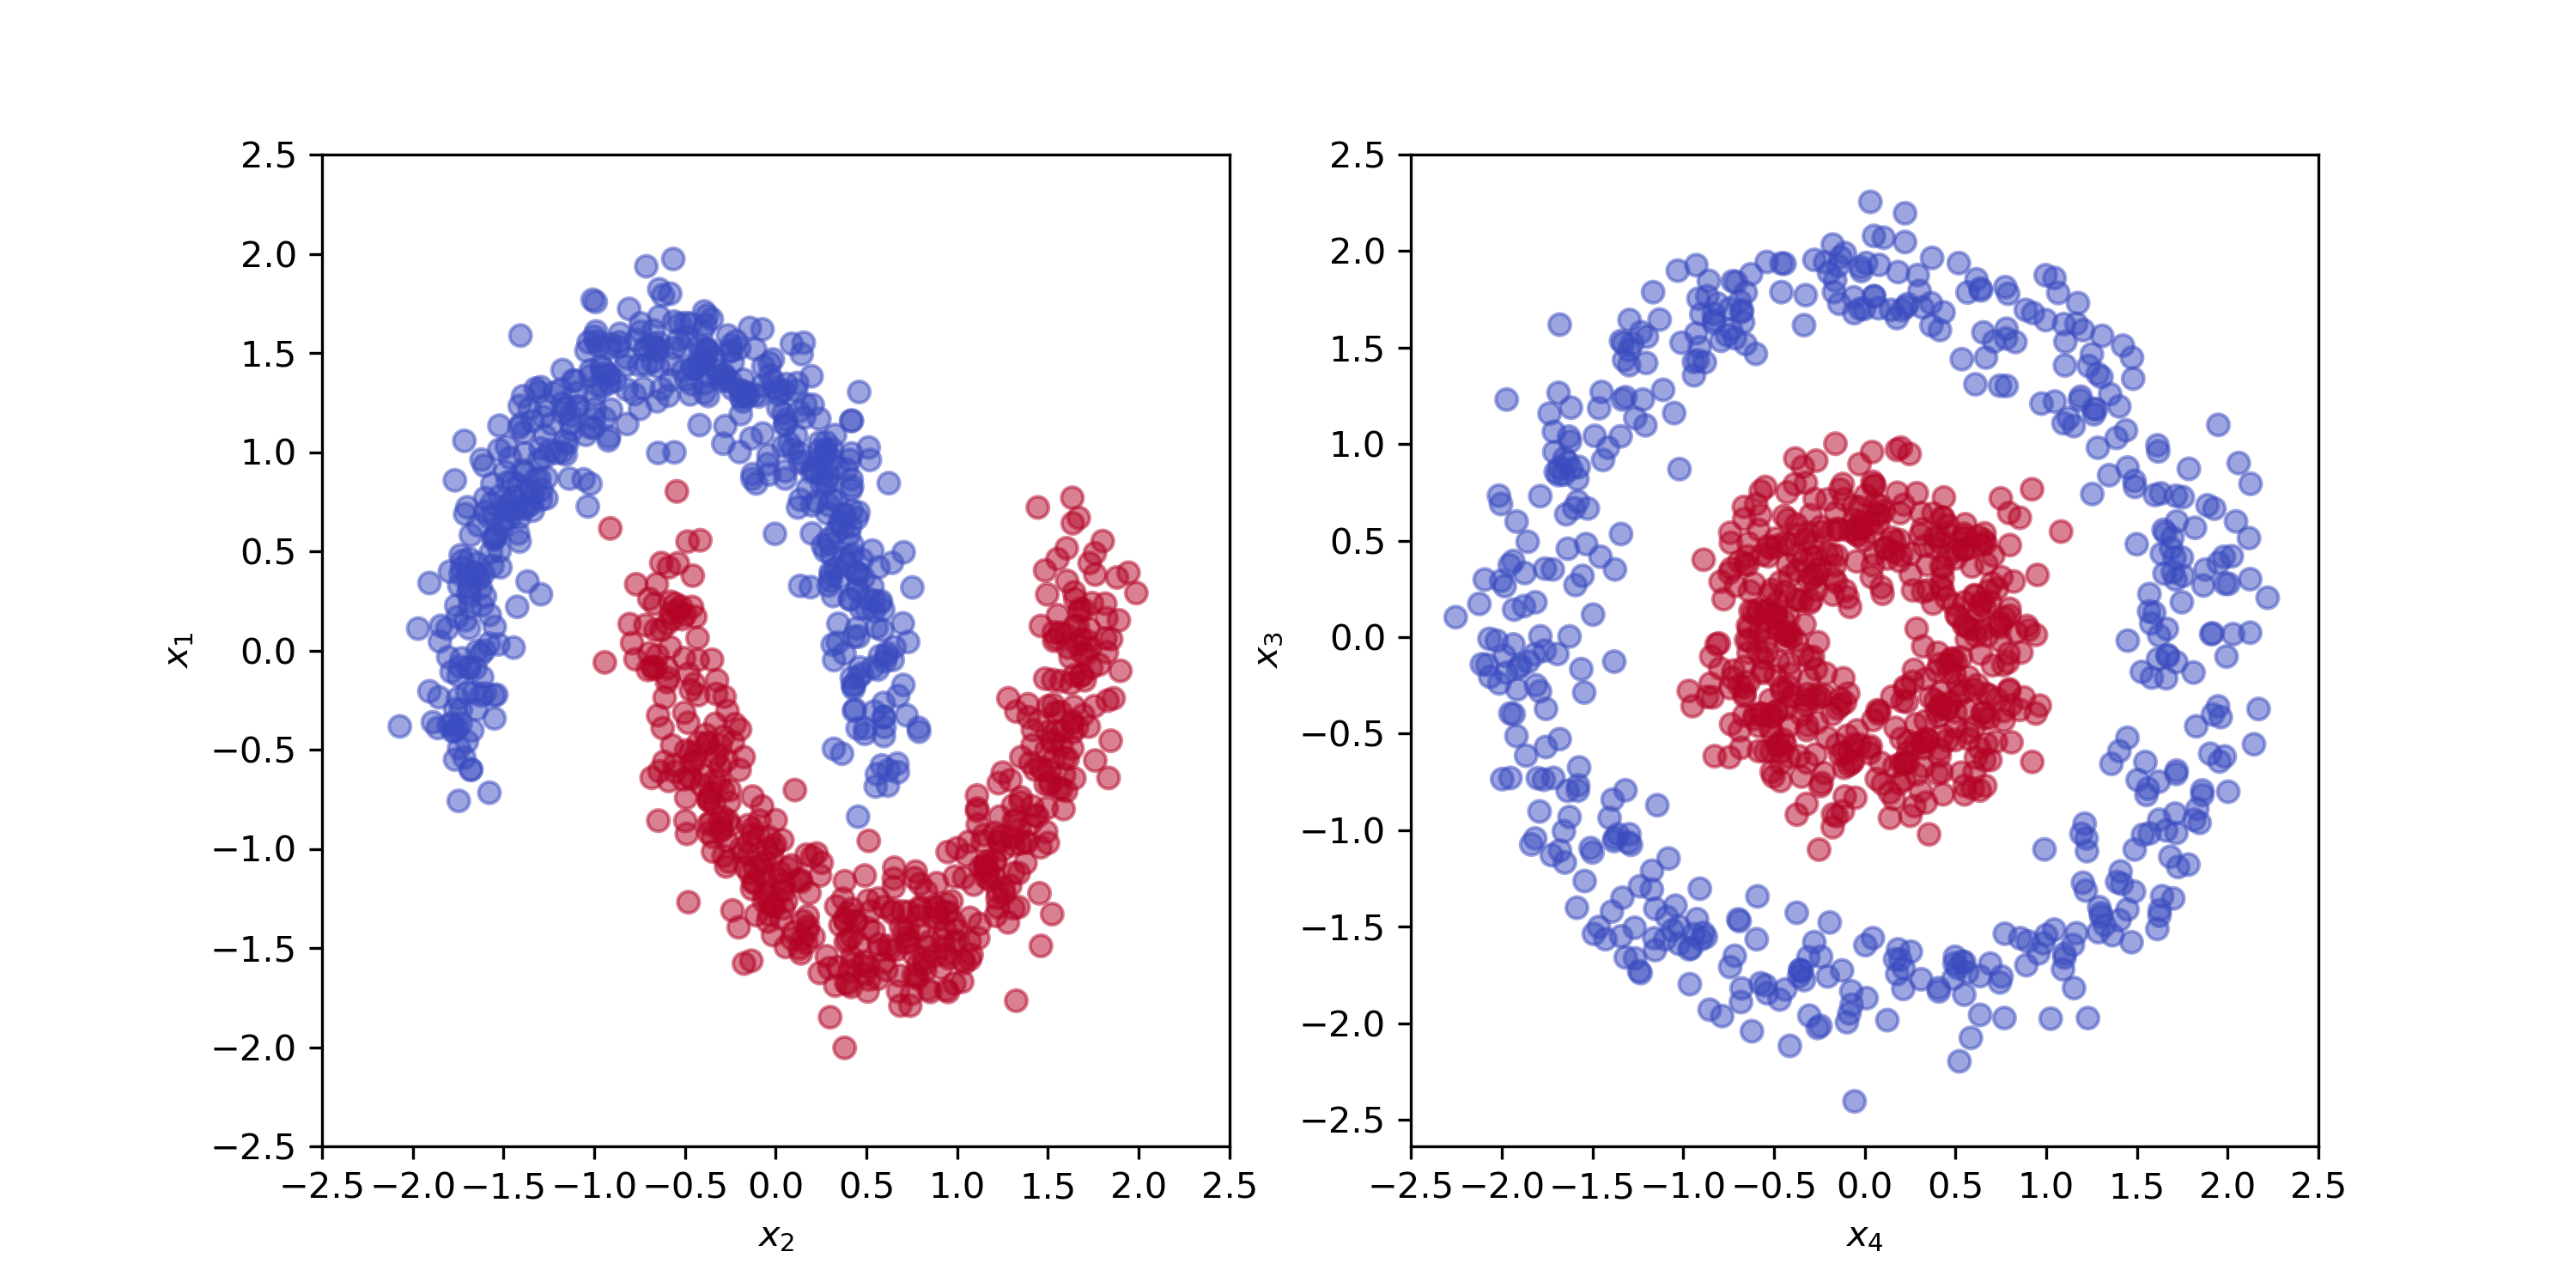
\includegraphics[width=1.0\linewidth]{moons-circles.png}
    \caption{This figure depicts the two dataset. On the left, the 'Two Moons Dataset' is displayed. On the right, the 'Circles' dataset. The datasets are normalized to have zero mean and unit variance in each feature.}
    \label{fig:moons_circles}
\end{figure}
The two selected datasets are the two moons dataset and the Circles dataset, depicted in Figure \ref{fig:moons_circles}.

Both datasets can be interpreted as a two dimensional plane, where the inputs describe coordinates of points on the plane. 
The labels of the dataset relates to the class.
Each point belongs to one class: red or blue.
Concretley, let $\begin{pmatrix} x_1 & x_2 \end{pmatrix}$ be the inputs of the two-moons dataset and $y_1 \in \{0,1\}$ the class label.
The data is generated by creating two half circles of evently spaced points, with a radius of $1$.
One of the half circles is rotated by 180 degrees and shifted by $0.5$.
Gaussian noise with a mean of $0$ and standard deviation of $0.1$ is added to each point in the dataset.

Let $\begin{pmatrix} x_3 & x_4 \end{pmatrix}$ be the inputs of the cirlces dataset and $y_2 \in \{0,1\}$ the class label.
The data is generated by creating evenly spaced points on the inner and outer circle. 
The center of both circles is at $(0,0)$ and the radius of the outer circle is $1$.
The radius of the inner circle is set to be $0.35$.
Gaussian noise with a mean of $0$ and standard deviation of $0.1$ is added to each point in the dataset.
The values of noise the size of the inner cirlce are selected, such that the points do not mix among the circles.

The classic machine learning library 'scikit-learn' is used to generate the data. 
The following code snippet demonstrates how the data was generated.
The described sampling strategy for the datasets relates to the content of the functions of 'scikitlearn', 'makemoons' and 'makecircles' respectively.

\begin{lstlisting}[language=Python]
    import sklearn
    # create the moons dataset
    moons = sklearn.datasets.make_moons(
        n_samples=2000, 
        noise=0.1
    )

    # create the circles dataset
    circles = sklearn.datasets.make_circles(
        n_samples=2000, 
        noise=0.1, 
        factor=0.35
    )
\end{lstlisting}

Since ranges of values of the datasets are different due to their sampling strategy, each feature is normalized individually to have zero mean and unit variance.
The final, normalized dataset is depicted in Figure \ref{fig:moons_circles}

To create a single dataset out of the two seperate datasets, the input features as well as the labels are concatenated.
Concretely, one sample of the concatenated dataset $\hat x$ contains one randomly selected sample from the two moons dataset and one randomly selected sample from the circles dataset.
The label $\hat y$ of the sample $\hat x$ also consist of the respective concatenated labels.
$$\hat x = \begin{pmatrix} x_1 & x_2 & x_3 & x_4 \end{pmatrix}$$
$$\hat y = \begin{pmatrix} y_1 & y_2 \end{pmatrix}$$

In this way, the whole dataset is concatenated.
Afterwards, the dataset is randomly split in half into a training set and a test set.
The result is a training set and a test set with 1000 samples each.

This dataset contains two seperate and indepdent tasks.
For each task, only the respective inputs contain valuable information for the prediction of the class.
To demonstrate this, the points each task are displayed however with the classes of the other task.
In all scenarios, there is no clear connection between the inputs and labels of the dataset.

Insert x1, x2 vs y2 ; x3, x4 vs y1

\subsection{The Model}
The neural network used to train on this task was inspired by the original lottery ticket experiments \autocite{DBLP:conf/iclr/FrankleC19}. A simple fully connected feed forward neural network was used.
Throughout this thesis the genreral architecture consists an input layer with four features ($x_1$ to $x_4$), two hidden layers of varyign sizes and one output layer with two features ($y_1$ and $y_2$).
All layers have ReLU activations and weights are initialized with Kaiming normal initialization \autocite{Kaiming} and biases are initialized with 0.

\subsection{The Algorithm}
With the dataset and architecture described above the aim was to find lottery tickets.
To accomplish this task, the classic Iterative Magnitude Pruning algorithm described in refIMP was employed used by \textcite{DBLP:conf/iclr/FrankleC19} in the original lottery ticket experiments.
The weights are rewound to $0$.
\textcite{LinearModeConnectivity} demostrated that the LeNet architecture trained on MNIST is stable at initialization, meaning that lottery can be found rewinding the weights to $t=0$ (the value at initialization). 
Since the model and dataset in our case is significantly less complex, it is assumed that the resetting the weights to zero is sufficient to discover lottery tickets.

As pruning criterion, the original Magnitude pruning used by \autocite{DBLP:conf/iclr/FrankleC19} is used. 
Since \autocite{DBLP:conf/nips/ZhouLLY19} showed that magnitude pruning is amongst the best performing criteria, it was selected due to its simplicity and widespread usage.
Biases are not pruned.

Contrary to \autocite{DBLP:conf/iclr/FrankleC19} where layerwise pruning is applied, the network is pruned globally.
Concretely, the pruning criterion is applied to all weights at once.
This enables the algorithm to 'select' the sparsity for each layer on it's own, resulting in less assumptions that have to be made.

One training run consists of $L$ pruning levels. 
At each pruning level, $p$-percent (pruning rate) of the remaining prunable parameters are set to zero.
The number of prunable parameters equals the number of weights that have not yet been pruned.
After $L$ pruning levels, the number of prunable parameters is termed the 'pruning target'.

Over the pruning levels, the number of prunable parameters goes from the initial number to the pruning target.
The sequence of prunable paremters is termed 'parameter trajectory'.
A parameter trajectory can be uniquely defined by 3 out of the following 4 values:
\begin{itemize}
    \item prunable parameters at initialization
    \item pruning levels
    \item pruning rate
    \item pruning target
\end{itemize}

Different combinations can be useful for different scenarios.

The networks are trained with the ADAM optimizer.
The learning rate is set to 0.001 and a batch size of 64 is used.
Further, throughout the experiments, early stopping is used to reduce the computational time.

As a pruning target, 112 weights was selected.
The pruning target is specified in absolute terms rather than as a percentage of the unpruned model, because several model sizes are used.
To select a pruning size, a small model was selected and evaluated to be trainable.
A model with 2 hidden layers with 8 neurons each, was selected and evaluated.
The pruning target refers to the number of prunable weights after all pruning iterations and not the number of active weights.
One could lower the pruning target even further, but the number of active weights can be significantly lower than the pruning target.
The model converges in less than 400 epochs and reaches almost $99.6$\% Accuracy.

INSERT TEST LOSS IMAGE, ACCURACY


\subsubsection{Network Splitting}
Since the goal of the experiments is to show if two seperate networks for inside the initial network, a mechanism to check if this is the case is needed.

Before the first pruning level, the network is converted into a Directed Acyclic Graph $\mathcal{G}$.
This graph representation is maintained throughout the pruning levels and updated after each level.

In the first step, each neuron is converted to a node in the graph.
Then each weight is converted into an edge that connects one node from the previous layer to the next layer.
All nodes, with the exception of the input layer, have biases associated with them.

Four categories are defined for the nodes and edges in the graph.
\begin{enumerate}
    \item active parameters  \\
    Nodes or edges in the graph that are connected to at least one input node and at least one output node.
    \item inactive parameters : \\
    Nodes or edges that are not connected to any output node. They do not influence the result of the network and they do not receive gradients. They can be removed.
    \item pruned parameters : \\
    Nodes or edges that have been masked out by the pruning algorithm.
    \item zombie parameters : \\
    Nodes or edges that are not connected to any input node, but are connected to at least one output node.
\end{enumerate}
Before the first pruning level, all nodes and edges are classified as 'active parameters'.
In the next step, each parameter in the graph will be assigned a category.
First, the newly pruned weights are extracted from the pytorch module.
Each edge in the graph that was pruned, is assigned that category.

Then, a subgraph $\mathcal{G}_{unpruned}$ is created, excluding all pruned weights.
On $\mathcal{G}_{unpruned}$, inactive nodes and edges are found and assigned their category.
All nodes that are not connected to any output node are classified as inactive.
Further, all edges that are connected to an inactive node are classified as inactive.

Then, a subgraph $\mathcal{G}_{active/zombies}$ is created, excluding all pruned and inactive weights.
On $\mathcal{G}_{active/zombies}$ zombie parameters are found and assigned to their category. 
All nodes that are not connected to any input feature are classified as a zombie parameter. 
Furhter, all edges that are connected to a zombie node are classified as a zombie parameter.

An active subgraph $\mathcal{G}_{active}$, where all nodes are connected to at least one input node and at least one output node.

\subsubsection{Matching Networks and Tasks}
The active graph $\mathcal{G}_{active}$ is used to find seperate components in the graph.
Conveniently, this can be done with a single networkx function.
\begin{lstlisting}[language=Python]
import networkx as nx

# G : nx.DiGraph
subnetworks = [
    G.subgraph(c) 
    for c in nx.connected_components(G.to_undirected())
]
\end{lstlisting}

Each node or edge of $\mathcal{G}_{active}$ is contained in exactly one of the subnetworks.
There is no overlap between the subnetworks.
Next, the subnetworks are matched to the tasks, which are defined by the dataset.
For each subnetwork and each task in the dataset, the inputs and outputs of the network are compared to the inputs and labels of the task.

Concretely, each task is associated with a set of inputs $T^{(i)}_{in}$ and a set of outputs $T^{(i)}_{out}$.
Further, each subnetwork contains a set of input nodes $N^{(j)}_{in}$ and a set output nodes $N^{(j)}_{out}$.

The intersection of the task inputs and the input nodes of the network denoted input coverage set $C^{(ij)}_{in}$ and output coverage set $C^{(ij)}_{out}$ for the outputs respectively.

$$
C^{(i,j)}_{out} = N^{(j)}_{out} \cap T^{(i)}_{out}
$$
$$
c^{(i,j)}_{out} = \frac{| C^{(i,j)}_{out} |}{|T^{(i)}_{out}|}
$$

$$
C^{(i,j)}_{in}  = N^{(j)}_{in}  \cap T^{(i)}_{in}
$$
$$
c^{(i,j)}_{in} = \frac{| C^{(i,j)}_{in} |}{|T^{(i)}_{in}|}
$$

For evaluating the coverage the the subnetworks as a whole, the number of paths from inputs to outputs are considered.
The total number of paths for a task is given by the product of the cardinatlity of the inputs set and the cardinality of the output set.
Similarly, the number of paths available in the subnetwork is given by the cardinality of theinput coverage set and the cardinatlity of the output coverage set.
The total coverage $c^{(i,j)}$ is defined as the ratio between the products.
$$
c^{(ij)} = \frac{
    | C^{(i,j)}_{in}| * | C^{(i,j)}_{out} |
    }{
    |T^{(i)}_{in}| * |T^{(i)}_{out}|
}
$$
The total coverage is 1 when the task is completely covered by the subnetwork.
It is 0, if either no input or no output of the task is covered by the subnetwork.
It is between 0 and 1, if at least one input and at least one output of the task is covered, but at least one input or output is not covered.
The total coverage is a useful indicator if all inputs and outputs are important, as they are counted equally.
In the case of the Moons-Circles Dataset, the total coverage is used.
For datasets where not all inputs or outputs are necessary or even desired to be used, the input coverage, output coverage or a combination thereof might be a more useful metric.

!!! Maybe move this to dataset.
!!! explain task description in dataset
!!! revise the math part. C is overloaded and number of tasks / subnetworks needs an identified. MAybe J, K and j, k for the running vars.

For instance, given the dataset in ref2, the dataset contains two tasks: the 'moons'-task and the 'circles'-task. 
The moons-task $T^{(1)}$ is associated with the inputs $T^{(1)}_{in} = \{x_1,x_2\}$ and the output $T^{(1)}_{out} = \{y_1\}$.
The circles-task $T^{(2)}$ is associated with the inputs $T^{(2)}_{in} = \{x_3,x_4\}$ and the output $T^{(1)}_{out} = \{y_4\}$.

The input, output or total coverage can be collected in a matrix $C$ of size $\tau \times j$, where $\tau$ is the number of tasks and $j$ the number of subnetworks. 
$c_{i,j}$ represents the value at the $i$-th row and the $j$-th column and $0 \leq c_{i,j} \leq 1$ holds.
Further, the sum of the matrix is upper bound by the number of tasks.
$$
\sum^{i} \sum^{j} c_{i,j} \leq \tau
$$


Given an unpruned network and a dataset with two tasks the matrix would look like the following 
$$
C = \begin{pmatrix}
    1 \\ 1
\end{pmatrix}
$$
Each task would be completely covered by the same network.
Since the network per definition covers all tasks before the first pruning level, the matrix will be a unit vector with as many entries as there are tasks.

After several pruning iterations, there network might contain two disconnected subnetworks.
In this case, an additional row is added to the matrix.
For instance, let the subnetworks perfectly match the tasks such that every task is completely covered by one subnetwork.
The matrix $C$ might look like the following.
$$
C = \begin{pmatrix}
    1 & 0 \\ 0 & 1
\end{pmatrix}
$$
After further pruning the network, all the connections to one of the input nodes might be pruned.
Then, one of the subnetworks would not be completely covered anymore.
Assuming there are one output node and two input nodes for task 1 and the subnetwork 2 covers all nodes except one input.
The resulting coverage would be 
$$
c^{(1,2)} =  \frac{
    | C^{(1,2)}_{in}| * | C^{(1,2)}_{out} |
    }{
    |T^{(1)}_{in}| * |T^{(1)}_{out}|
} = \frac{1}{2}
$$
and the resulting matrix $C$ would look like the following

$$
C = \begin{pmatrix}
    1 & 0 \\ 0 & 0.5
\end{pmatrix}
$$

If the sum of $C$ is equal to the number of tasks and the number of subnetworks is equal to the number of tasks, then the network is perfectly split.

If the sum of $C$ is equal to the number of task, but there are less subetworks than tasks, the network still needs to split.
The number of splits that are required can is the difference between the number of tasks and the number of subnetworks.

If the sum of $C$ is less than the number of tasks, the network already has lost at one input or output.
This scenario will be referred to as a 'degraded' network.
Once a network is degraded, it is impossible that a perfect split is reached.
In the case of the Moons-Circles dataset, the training is stopped as soon as the network is degraded to save computational resources.

(additional)
For mnist, we use the output coverage, since it is expected that the network will come to ignore inputs.
Then the output coverage is used. Also between 0 and 1 . Works the same way as with the total coverage in the previous case.

\subsubsection{Model Extension}
A technique used to create models that are comparable on the basis of prunable parameters is termed 'model extension'. First, the problem is described which model extension is intended to solve, then the technique is described in detail.

To compare networks over pruning levels, a significant quantity is the number of prunable parameters the networks has left at each iteration.
For instance, comparing two networks with 1000 and 1200 prunable parameters in the beginning, 6 pruning levels and a pruning rate of $0.2$, the following parameter trajectories $t_{1000}$ and $t_{1200}$ would form.
$$
t_{1000} = [1000, 800, 640, 512, 409, 327, 262]
$$
$$
t_{1200} = [1200, 960, 768, 614, 491, 393, 314]
$$
The first problem is that the pruning target is not aligned.
Therefore, let the pruning rate be variable and the pruning target is fixed.
The pruning rate can be calculated with 
$$
p = 1 - \sqrt[L]{\frac{T}{P}}
$$
where $L$ is the number of pruning levels, $P$ equals the number of prunable parameters before pruning and $T$ denotes the pruning target.

Let the pruning target be $200$ with 6 pruning levels.
The pruning rates are $p_{1000} = 0.235$ and $p_{1200} = 0.258$ respectively.
The resulting parameter trajectories are as follows.
$$
t_{1000} = [1000, 764, 584, 447, 341, 261, 200]
$$
$$
t_{1200} = [1200, 890, 660, 489, 363, 269, 200]
$$

With this change, the pruning targets are aligned and are comparable.
However at no point during the trajectory values are aligned.
For instance, the network that has $1000$ prunable parameters in the beginning might split after iteration 5, where it has $341$ prunable parameters left. 
The other network might split at iteration after 6, where it has $269$.
However, since they are not aligned one cannot ignore the possibility that the second network would also have split at $341$, but not at $363$. 
The second network would only split earlier if it would split with 22 additional parameters.
When scaling up networks, the intervals at which the had the possibility to split are spaced further from each other, making this effect even more pronounced.

Ideally, different networks would have parameter trajectory that are shared, such that they can be compared at every step.
To achieve this on can 'extend the model'.

Let a network with $n$ prunable parameters be the base of the extension.
The network is pruned for any number of pruning levels with a given pruning rate $p$.

TODO: write about model extension.

Extending the model means to add parameters to the model, such that pruning it once with the set pruning rate would result in the same number as paraemter